\chapter{Implementation}
Before being able to develop a second working prototype that implements some of the functionality, it is needed a fully functional back-end component. This chapter describes how this was achieved with the selected design and technological choices going from the development of each back-end component to the development and implementation of a second and a third prototype.
\section{Back-end implementation}

\subsection{Database}
Dynamo was the chosen database as justified in the design chapter. It is a schema-free database that only requires a table name and a primary key. The primary key can be composed of up to two attributes, in which case the first attribute defines the partition range and the second attribute defines the sorting over that partition. Dynamo is extremely efficient when used in the correct way. 

Designing the table to contain the air quality readings is straightforward. The key is composed of the unique ID of the fixed sensor being the partition key, and the updated hour being the partition sort key. This provides the advantage that all the readings of a specific sensor can be retrieved together and that they will be dispatched sorted, saving computing time on the client. Other general usage tables are also created to contain the coordinates of all sensors, and the COMEAP thresholds for each pollutant. These tables contain at most 20 items and are designed to be retrieved as a whole, so there is no need to sort them on a second attribute.

\subsection{Web crawler and daemon}
A web crawler is a service that automatically browses the web and extracts useful information to insert it later into a persistent storage. The air quality data needed to feed the application will be extracted from the Air Quality in Scotland website using scrappy as discussed in previous chapters. The way scrappy extracts structured data from a webpage is by browsing the HTML document with XPATH expressions. 

\begin{figure}[H]
\begin{adjustbox}{width=.5\textwidth,center=\textwidth}
  \centering
  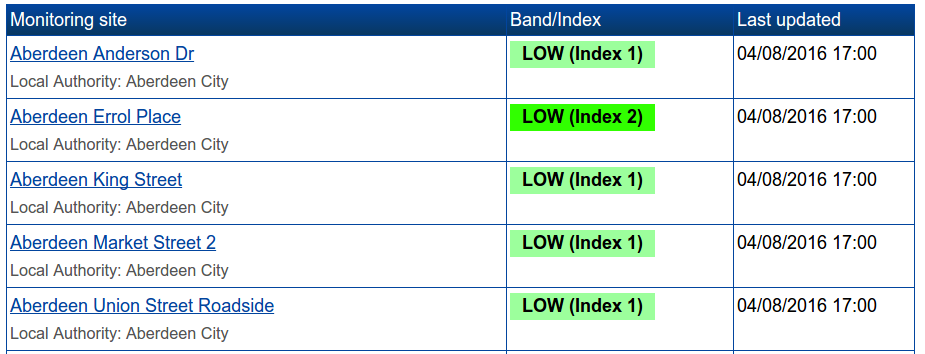
\includegraphics[scale=1]{images/monitoring_summary.png}
\end{adjustbox}
  \caption[Pollution sensors list]{Pollution sensors list \footnotemark}
  \label{fig:pollution_sensors_list}
\end{figure}
\footnotetext{\url{http://www.scottishairquality.co.uk/latest/summary}}

The website data source contains sensors from different locations in Scotland as shown in Figure \ref{fig:pollution_sensors_list}. The first thing the crawler would need to do is to extract the links to navigate through all the available sensors. The rendered sensor list table looks like the code bellow in plain HTML. It is noticeable that the XPATH selector needs to go through the table to reach the \textit{href} attribute to access the data for that particular sensor.

To select the \textit{href} attribute: \bigskip

{\centering
\begin{BVerbatim}
//tr/td[1]/a@href
\end{BVerbatim}
\par
}\bigskip

The output of the XPATH selector is highlighted in red: 

\begin{Verbatim}[fontsize=\small,commandchars=\\\(\)]
<table>
  <tbody>
    <tr>
      <td><a href="(\color(red)site-info?site_id=ABD1")>Aberdeen Anderson Dr</a><br></td>
      <td><span>LOW (Index 1)</span></td>
    </tr>
      <tr>
      <td><a href="(\color(red)site-info?site_id=ABD)">Aberdeen Errol Place</a><br></td>
      <td><span>LOW (Index 2)</span></td>
    </tr>
  </tbody>
</table>
\end{Verbatim}

Once that the URL containing the data is extracted, scrappy executes another request to select the interesting data for each sensor. The readings are rendered through a table which contains the pollutant, the band, the concentration and the update period as shown in Figure \ref{fig:pollution_site readings}

\begin{figure}[H]
\begin{adjustbox}{width=.5\textwidth,center=\textwidth}
  \centering
  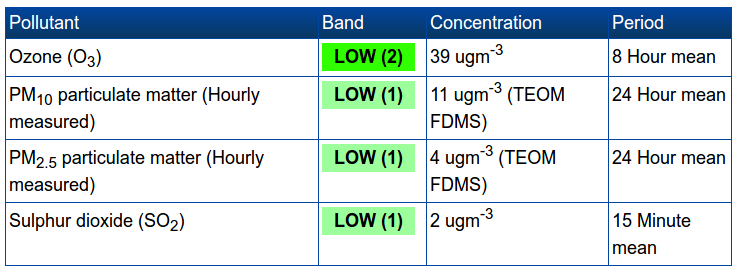
\includegraphics[scale=1]{images/site_readings.png}
\end{adjustbox}
  \caption[Edinburgh St Leonard's site readings]{Edinburgh St Leonard's site readings \footnotemark}
  \label{fig:pollution_site readings}
\end{figure}
\footnotetext{\url{http://www.scottishairquality.co.uk/latest/site-info?site_id=ED3}}

To extract the pollutants information contained in the the table all the \textit{td} elements are selected: 

{\centering
\begin{BVerbatim}
td[1]
\end{BVerbatim}
\par
}\bigskip

The output of the XPATH selector is highlighted in red: 

\begin{Verbatim}[fontsize=\small,commandchars=\\\(\)]
<table>
  <tbody>
    <tr>
      <td>(\color(red)Ozone (O<sub>3</sub>))</td>
      <td>(\color(red)LOW (2))</td>
      <td>(\color(red)39 ugm<sup>-3)</sup></td>
      <td>(\color(red)8 Hour mean)</td>
    </tr>
  <tr>
    <td>(\color(red)PM<sub>10</sub> particulate matter (Hourly measured))</td>
    <td>(\color(red)LOW (1))</td>
    <td>(\color(red)11 ugm<sup>-3</sup> (TEOM FDMS))</td>
    <td>(\color(red)24 Hour mean)</td>
  </tbody>
</table>                
\end{Verbatim}

Following the same principle, the remaining meta-data such as the reading time-stamp and the sensor details are extracted. Still, the data is not in the optimal format yet; some readings contain embedded HTML tags that need to be cleaned before any insertion in the database. Fortunately, scrappy provides a pipeline process before exporting the data into the desired format. The cleaning process is straightforward, by cropping the undesired tags with python strings processing. 

Once the data is ready to be exported, it is translated into a Python \textit{dict} and inserted right-away in the dynamo table: \bigskip

{\centering
\begin{BVerbatim}
        table.put_item(Item = dict(sensor_reading))
\end{BVerbatim}
\par
}\bigskip


The described above python script will be executed constantly to keep the data as up to date as possible. Unix systems have a built-in daemon utility that can be used to execute the script directly called Cron. This service reads a Crontab file containing the information of the all the scheduled tasks. To add an entry to the crontab file and indicate that the Crawler script will be executed every 30 minutes, the following command is executed: \bigskip

{\centering
\begin{BVerbatim}
        */30 * * * * python crawler.py
\end{BVerbatim}
\par
}

\subsection{Advice service}
The advice service will respond the requests from the Android device to provide the personalised health advice as discussed in previous chapters. It is composed of two components: an expert system and a Java servlet to expose the service through HTTP GET requests. 

The first task is to translate the advice offered by the COMEAP report into rules to form a knowledge base. This knowledge base will live in the memory of the Java web container and whenever it receives new queries it will infer the advice from the asserted facts. The facts representing the advice are like \textit{if-else} statements that focus on three conditions: the pollution level index, the sensitivity of the person and the age of the person. 

The Jess engine allows to define templates, which are like java classes that describe how a statement should look like when asserted. The actual values contained by the fact are named slots. These templates are useful to describe the conditions that are needed to assert an advice. For instance, the templates \textit{pollutionLevel} and \textit{person} can be defined in the following way: 

{\centering
\begin{spverbatim}
(deftemplate pollutionLevel
    (slot value)
)

(deftemplate person
    (slot age)
    (slot sensitivity); The possible values are 1 and 2.
)
\end{spverbatim}
\par
}

The logic in Jess is modelled with rules. They define the conditions or facts that should be fulfilled in order to assert a new fact. The following rule is an example that models the COMEAP advice given to adult sensitive individuals when the air quality index is at a level between 4 and 6 points. If all these conditions are fulfilled then it is possible to assert the advice: "Consider reducing strenuous physical activity, particularly outdoors". 

{\centering
\begin{spverbatim}
(defrule consider_reducing_strenuous_activity_sensitive_4_6
    ?per <- (person {sensitivity >= 2})
    ?per <- (person {age >= 65})
    ?pol <- (pollutionLevel {value >= 4 && value <= 6})
    =>
    (assert
        (advice (text "Consider reducing strenuous physical activity, particularly outdoors")))
)
\end{spverbatim}
\par
}
The rule engine is initialized in the context of the Java Enterprise web container, and the facts are loaded from a \textit{facts.clp} file to ease the way they can be later modified. 

To grant Android access to the advice assertions, the inference engine is exposed in a public domain on the Amazon infrastructure. The running servlet handles all incoming \textit{get} request asking for the advice service. The client has to append the age, the sensitivity and the pollution level variables to the \textit{http get} request in the form of query parameters as in the following example: \bigskip

{\centering
\begin{BVerbatim}
http://.../Advice/advice?age=?&sensitivity=?&airQualityIndex=?
\end{BVerbatim}
\par
}

\section{Front-end implementation}
\subsection{Access to air quality data}
Once the services are available to query, the connection between the device and the air quality data hosted on dynamo has been implemented. Amazon makes available an Android library ready to connect to the database readings\footnote{\url{https://aws.amazon.com/mobile/sdk/}}, it is included as a dependency in the Android project. In order to handle and represent the database entries in Android, Plain Old Java Objects \textit{POJO's} have been defined. They are simple classes that describe the general structure and contents of a persisted data reading. An example is the following \textit{SensorReading}, which represents the raw \textit{JSON} database reading  and contains a list of the available pollutants, the date it was last updated, and the air quality index:

{\centering
\begin{spverbatim}

@DynamoDBTable(tableName = "airquality_readings")
public class SensorReading {

    private HashMap<String, Pollutant> pollutants = new HashMap<>();
    private String lastUpdated;
    private String airQualityIndex;
}
\end{spverbatim}
\par
}

This eases the way the data is queried from the device, allowing to define a \textit{DatabaseManager} to retrieve the readings in the following way: 

{\centering
\begin{spverbatim}
public List<SensorReading> getReadingsBySourceID(String sourceID, String since, String to) {

  Condition rangeKeyCondition = new Condition().
    withComparisonOperator(ComparisonOperator.BETWEEN.toString()).
    withAttributeValueList(new AttributeValue().
    withS(since), new AttributeValue().withS(to));

  DynamoDBQueryExpression<SensorReading> queryExpression = new
    DynamoDBQueryExpression().
    withHashKeyValues(sourceID).
    withRangeKeyCondition("lastUpdated", rangeKeyCondition);
  
return dynamoDBMapper.query(SensorReading.class, queryExpression);
}
\end{spverbatim}
\par
}

\subsection{Localizing the closest sensor reading}
Because many sensors may be available to query, the closest sensor should be identified and displayed. To provide localisation features to the application, it should inform that it has the intention to use such features before installed. To do so, the permission is added to the project \textit{manifest.xml} in the following way: \bigskip

{\centering
\begin{BVerbatim}
<uses-permission android:name="android.permission.ACCESS_COARSE_LOCATION"/>
\end{BVerbatim}
\par
}
\bigskip

Once that the location permissions have been granted, the application retrieves the last sensed location by the device and a list including all available sensors and their locations from the Dynamo database. The task is to find out the closest sensor given the full coordinate list and the current location, which is also in longitude-latitude format. The nearest sensor is chosen by calculating the distance between all options using the distance between two points formula: 

\begin{equation}
d={\sqrt {(\Delta x)^{2}+(\Delta y)^{2}}}={\sqrt {(x_{2}-x_{1})^{2}+(y_{2}-y_{1})^{2}}}.\,
\end{equation}

\subsection{Libraries and custom components}
Many android UI components like buttons, bars or windows are already built and made available for public usage. Because crafting all the interface components from scratch is an extensive time-consuming task, most UI components were outsourced. Just in very specific cases where no component was found suitable, it was developed from scratch. 
The following public libraries were used to construct the UI:
\begin{itemize}
    \item Deco view charting \footnote{\url{https://github.com/bmarrdev/android-DecoView-charting}}: Provides components to create animated circular charts.
    \item MPAndroidChart \footnote{\url{https://github.com/PhilJay/MPAndroidChart}}: Provides components to create many different types of charts: lines bar and pie charts among others.
    \item Android simple tooltip \footnote{\url{https://github.com/douglasjunior/android-simple-tooltip}}: Provides a tool-tip component.
	\item Material date-time picker \footnote{\url{https://github.com/wdullaer/MaterialDateTimePicker}}: A built-in calendar to select time and date.
  \item Round corner progress bar \footnote{\url{https://github.com/akexorcist/Android-RoundCornerProgressBar}}: A fancy fully configurable progress bar.
\end{itemize}

\section{Second Prototype}
Now that the back-end is implemented to serve the application and that all the Android components are in place, it is possible to describe the second prototype with some working capabilities, like retrieving and rendering real data from the cloud services. This prototype will follow the established on previous chapters but providing a real interactive experience in order to get feedback from users and make improvements before releasing the third prototype. 

\begin{figure}[H]
\begin{adjustbox}{width=1.2\textwidth,center=\textwidth}
  \centering
  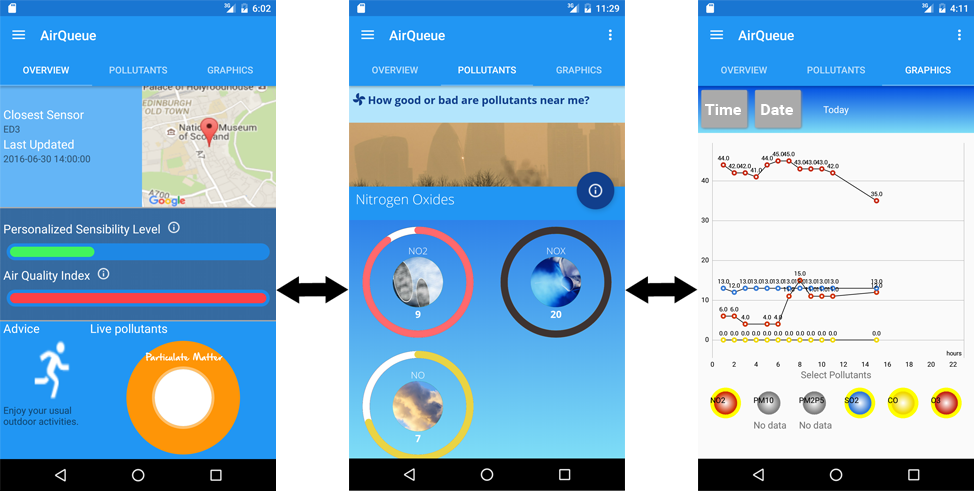
\includegraphics[scale=1]{images/secondPrototype.png}
\end{adjustbox}
  \caption[Second prototype]{Second prototype. From left to right: first, second and third visualization.}
  \label{fig:first_second_prototype}
\end{figure}

\subsection{First visualization}
At the top of the screen information of the air quality sensor is rendered employing text and a map. The map is retrieved by coordinates using the Google Maps API\footnote{\url{https://developers.google.com/maps/}}. In the centre there are two progress bars, one serves to adjust the personalised sensitivity level, and another one shows the current air quality index. The bottom components are including the personalised health advice, and the available pollutants at this time (In figure \ref{fig:first_second_prototype} the only pollutant available is particle matter). 

At this iteration, the colour choices are starting to be defined, yet they are not perfect but provide guidance on what is wanted. The colour that is desired to be predominant is blue because it evokes to fresh air. There are separators within the screen to indicate that the sections accomplishes different functions and to guide the user through its learning. Also, the font choices pretend to provide readable text. 

\subsection{Second visualization}
This visualisation as previously stated aims to give an understandable first insight of the current pollution at a particle level. At this iteration is considered to include all particles in 'spheres' which contain the reading rendered in a circular graph that changes in colour and arc coverage according to the reading. The pollutants are grouped per category, in the Figure \ref{fig:first_second_prototype} are shown pollutants known as nitrogen oxides. Furthermore, images are included to allow the user to identify the current category and particle with ease.

To accomplish the second sub-requirement which is including further information about the pollutant when clicked, a second sub-screen was added. This one contains simple textual information about the pollutant sources and its associated health effects as shown in Figure \ref{fig:second_visualization_sub_screen}. 

\begin{figure}[H]
\begin{adjustbox}{width=.3\textwidth,center=\textwidth}
  \centering
  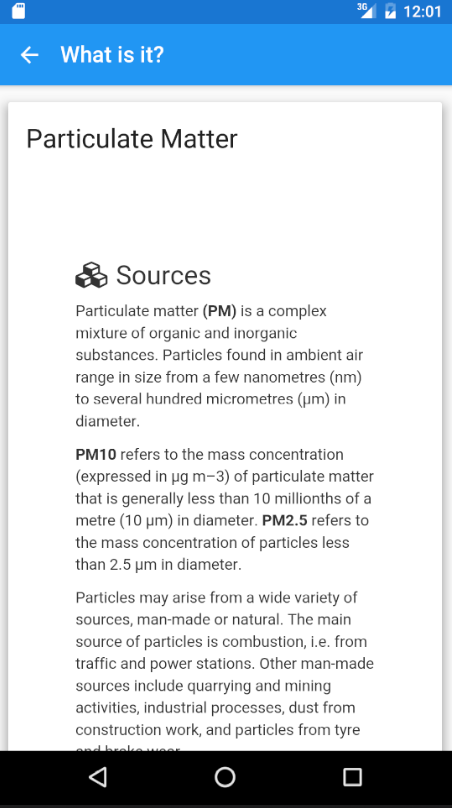
\includegraphics[scale=1]{images/second_visualization_sub_screen.png}
\end{adjustbox}
  \caption[Pollutant sources and effects screen]{Pollutant sources and effects screen}
  \label{fig:second_visualization_sub_screen}
\end{figure}

\subsection{Third visualization}
The third visualisation includes the particles over defined periods of time using a line graph. The x-axis represents the time while the y-axis represents the reading. The user is able to select the data on specific dates and hours by using the available date and time buttons. At this iteration it was decided that the user would be able to overlap different pollutants and render them simultaneously on the same graph, this is done by selecting the pollutants on the bottom. Also, different colours are associated with the pollutants to be able to recognise them in the graph.

\section{Third prototype}
For the making of a third prototype, there were small inner evaluations with different users and stakeholders as mentioned in the Methodology section. Their feedback was taken into account to discover what was failing with the second iteration and improve this final prototype. 

\begin{figure}[H]
\begin{adjustbox}{width=1.2\textwidth,center=\textwidth}
  \centering
  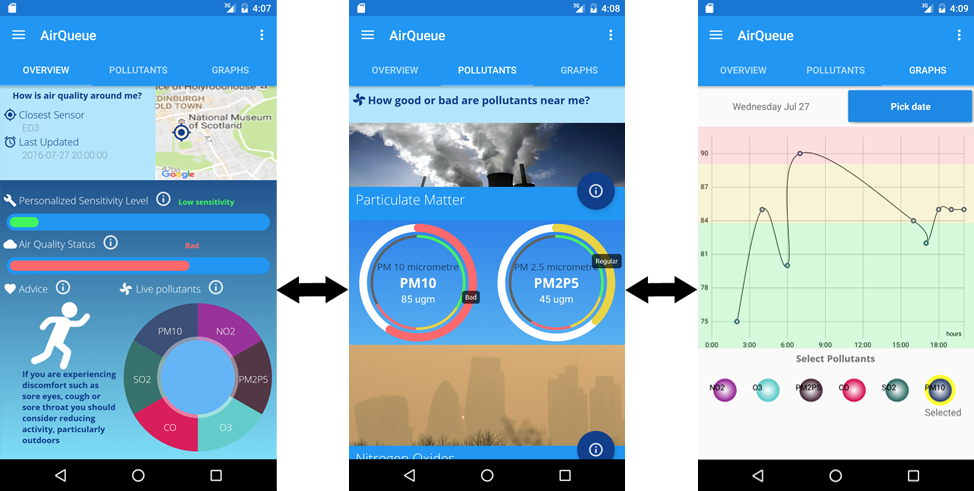
\includegraphics[scale=1]{images/thirdPrototype.png}
\end{adjustbox}
  \caption[Second visualization sub-screen]{Second visualization sub-screen.}
  \label{fig:third_prototype}
\end{figure}

\subsection{First visualization}
The findings from evaluating the second version of this screen were that the overall usability of the interface was not high nor low. People could use the interface after few attempts by playing around, but they were sometimes confused about what the elements were doing, and how to use them. Because of this, the interface was improved to achieve a better learn-ability through changing the arrangement of the elements, the colours and adding other indicative visual and textual elements.
The improvements with respect the past iteration were the following:
\begin{itemize}
    \item  The way the interface is sectioned was changed. Having three sections was leading for confusion rather than for guidance.
    \item Background colours were changed to allow the components to be more distinguishable employing one primary colour in the top, and one gradient in the bottom.
    \item  The three three colours used in this screen blend better to avoid distracting the user.
    \item Indicative icons were added to provide usability. It is now easier to learn how to navigate through the interface.
    \item Info buttons with tooltips were added. They give further information about what is happening with a particular screen component. For instance, they say how to adjust the personalised sensitivity level, or where does the air quality status comes from. This to provide confidence. 
    \item Text fonts were richly improved, using the Google recommended fonts when appropriate:  Open-Sans and Robotto.
\end{itemize}

\subsection{Second visualization}
The second iteration of this screen was not very hard to use overall; the users were able to navigate through this interface with ease. On the other hand, feedback also showed that there were too many images leading to distraction. 

The improvements with respect the past iteration were the following:
\begin{itemize}
    \item The images in the centre of each pollutant were confusing rather than accomplishing an associative function. They were removed.
    \item Apart from the associative colours in the circular graph (green, yellow, red) a textual tag was included (good, regular, bad).
    \item The titles of the pollutants were expanded, as they were not very distinguishable. 
    \item An inner smaller circle explaining the thresholds for each pollutant through traffic light colours was added to the circular graph. 
    \item Text fonts were richly improved, using the Google recommended fonts when appropriate:  Open-Sans and Robotto.	
\end{itemize}

\subsection{Third visualization}
From evaluating this screen, it was encountered that users were finding hard to manipulate more than one pollutant at a time. Also, the specific time selectors were very cumber-stone requiring the user to perform many steps to achieve the rendering of the interface. 
The improvements with respect the past iteration were the following:
\begin{itemize}
    \item The colours were changed avoiding colours similar to the already used ones in the semaphore scale to elude the user to associate the pollutants state with them. They were also tied with the colours of the same pollutants in the first visualisation to ease the learning process.
    \item The number of possible selected pollutants was limited to one. As they were hard to distinguish together in the same line graph. 
    \item The selector by time was removed, leaving the date selection alone. The reason for this is that the readings outside the threshold of a day were very hard to represent and read, and it was cumber-stone to select the specific time ranges. 
    \item An indicative overlay was added behind the line graph. Showing the acceptance level at which the current reading was located in the semaphore color scale. 
\end{itemize}

\section{Deployment}
At this point, the development of the third prototype was exhausted. The back-end component has been working nonstop since the 15th of June and gathered more than 55,000 readings containing more than 220,000 pollution readings from sensors spread all over Scotland. There is an added value for providing the application for public download and usage and it enables further testing and feedback that goes beyond a couple of users.

\begin{figure}[H]
\begin{adjustbox}{width=.8\textwidth,center=\textwidth}
  \centering
  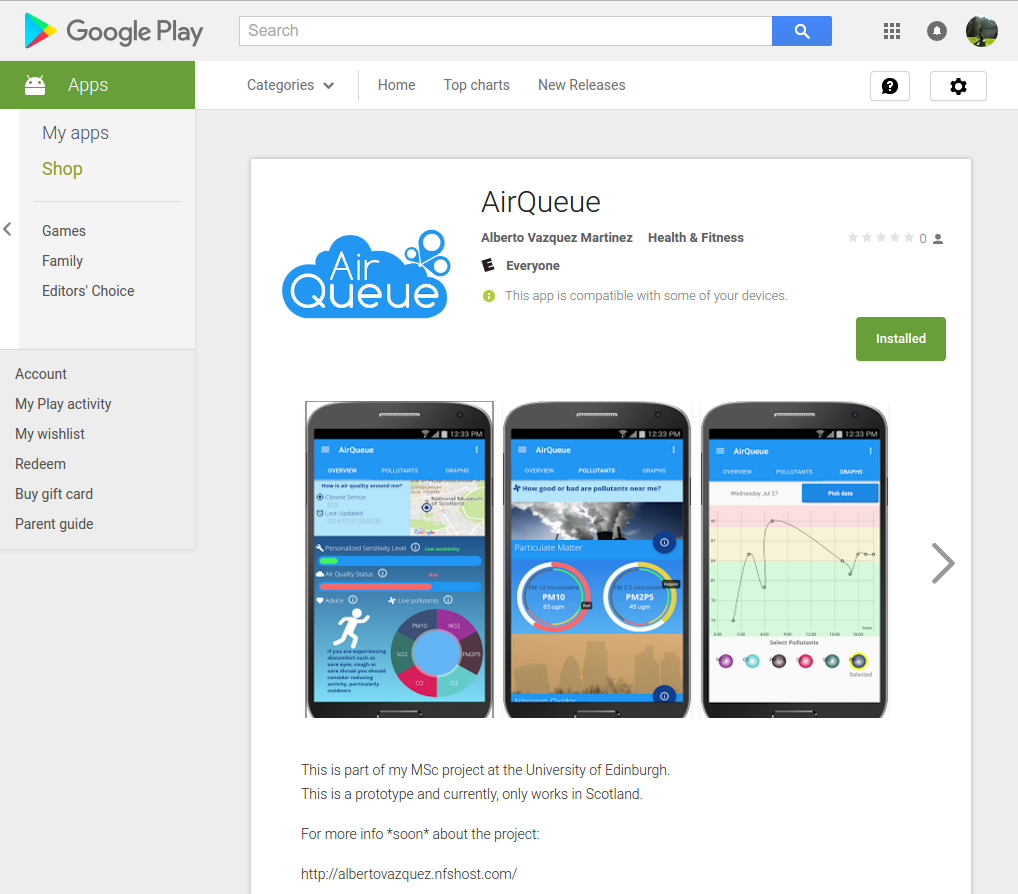
\includegraphics[scale=1]{images/play_store.png}
\end{adjustbox}
  \caption[Deployment on Google Play Store]{Deployment on Google Play Store.\footnotemark}
  \label{fig:deployment_play_store}
\end{figure}\footnotetext{\url{https://play.google.com/store/apps/details?id=com.beto4812.airqueue&hl=en_GB}}

